\clearpage
\section{Lokální oscilátor}
%\subsection{Princip DDS}
\indent\indent Lokální oscilátor je postaven na obvodu od firmy Analog Devices AD9850BRS. Jedná se o takzvaný DDS - Direct Digital Synthesizer (přímá digitální syntéza) což je technologie určená pro generování, většinou harmonických signálů s digitálně přesně nastavitelným výstupním kmitočtem. Obvod AD9850 dokáže generovat, za předpokladu referenčního hodinového signálu o frekvenci $125~MHz$, sinusové průběhy od $0,0291~Hz$ s krokem $0,0291~Hz$. Integrovaný obvod se skládá z: rozhraní pro konfiguraci, registru pro zachycení vstupních dat, registru pro aktuální konfiguraci, DDS bloku, DAC a nízkošumového komparátoru.

Jak vlastně DDS funguje? DDS je tvořena pamětí nejčastěji ROM (Read Only Memory) ve které jsou uchovány vzorky funkce, kterou chceme generovat. V případě AD9850 jsou vzorky v rozlišení 10 bitů. Hodnota ve fázovém registru určuje o kolik vzorků se při dalším taktu referenčních hodin přesune. Když vnitřní čítač dosáhne konce paměti, dojde k jeho vynulování a pokračuje opět od začátku. Data z paměti jsou přiváděna  do rychlého 10 bitového DA převodníku, kde se převádí na napětí.  			
  			
DDS Obvod se podle obdrženého konfiguračního slova nastaví do odpovídajícího módu a pokud jsou konfigurační data v pořádku, je na výstupu DA převodníku požadovaný signál odpovídající nastavenému kmitočtu.

% blokáč AD9850
\begin{figure}[H]
	\centering
	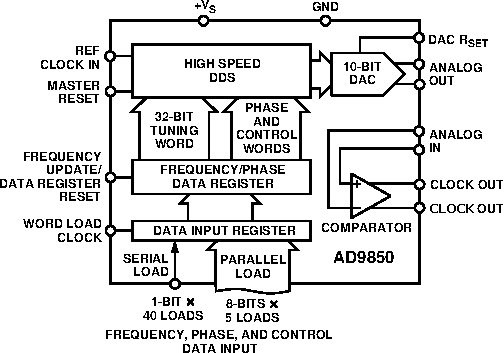
\includegraphics[width=140mm]{img/lo/AD9850_bd.pdf}
	\caption{Blokové schéma AD9850}    		
\end{figure}

\clearpage

\subsection{Výpočet konfiguračního slova}
\indent\indent Konfigurační slovo má 40 bitů a slouží k nastavení výstupní frekvence a módu práce DDS. První 4 byte určují požadovaný kmitočet a poslední byte určuje mód. Hodnota 32b slova pro konfiguraci frekvence se vypočítá podle vztahu:
  			$$f_{OUT} = \frac{\Delta Phase \cdot CLKIN}{2^{32}}$$
  			
  			\hspace*{2cm}kde:\newline    
  			\hspace*{4cm}$f_{OUT}$ \dotfill požadovaná výstupní frekvence\hspace*{4cm}\newline
		  	\hspace*{4cm}$\Delta Phase$ \dotfill 32b konfigurační slovo\hspace*{4cm}\newline
		  	\hspace*{4cm}$CLKIN$ \dotfill frekvence referenčních hodin\hspace*{4cm}\newline
		  	
		  	
		  	Poslední byte konfiguračního slova přepíná DDS do čtyřech módů práce:
		  	
		  	\begin{table}[H]
    			\begin{center}
    				\caption{Možné módy obvodu AD9850}
      				\label{tab:lo_mod}      
					\begin{tabular}[H]{!{\vrule width 1pt}c|c!{\vrule width 1pt}}
				        \specialrule{1pt}{0pt}{0pt} 
				        \textbf{Hodnota} & \textbf{Popis} \\\specialrule{1pt}{0pt}{0pt} 
				        $4$ &	power-down	\\\hline 				
				        $0$ &	power-up	\\\hline 
				        $2$ &	test		\\\hline 
				        $1$ &	test
						\\\specialrule{1pt}{0pt}{0pt}         
		    		\end{tabular}     				
    			\end{center}
  			\end{table}
  			
  			Když je tato posloupnost vytvořena, tak je buď pomocí sériového nebo paralelního rozhraní nahrána do DDS.

\subsubsection{Konfigurace DDS}
\indent\indent Aby AD9850 správně fungoval, je třeba jej napřed správně nakonfigurovat. K tomuto účelu je možné přistupovat dvěma způsoby. První způsob je pomocí paralelního rozhraní a druhý pomocí rozhraní sériového.
  		
\subsubsection{Konfigurace pomocí paralelního rozhraní}
\indent\indent Ke konfiguraci se používá 8 bitového datová sběrnice pro přenos dat, k ovládání komunikace slouží řídící signály: WRITE, FQ\_UD a RESET. Komunikace probíhá po jednotlivých bytech. Napřed je třeba obvod resetovat. To se provede přivedením logické úrovně H na signál RESET po dobu minimálně pěti period referenčních hodin. Tím se vynuluje ukazatel registru zachycení a DDS je připravena k zápisu konfiguračního slova. Konfigurační slovo o délce 40b neboli 5B je posloupnost určující výstupní frekvenci,  fázi a mód. Zápis probíhá tak, že na datovou sběrnici nastavíme byte (začíná se od LSB směrem k MSB). Poté vyšleme zapisovací impuls na signál WRITE široký minimálně $3,5~ns$. Data jsou zapsána do záchytného registru pro konfiguraci při náběžné hraně. Poté počkáme minimálně $3,5~ns$ (během tohoto času se zvyšuje ukazatel do záchytné paměti vstupních dat) a můžeme pokračovat. Tento proces je nutné zopakovat celkem pětkrát aby se celé konfigurační slovo přeneslo do DDS. Nakonec se celé konfigurační slovo uloží do řídícího registru DDS. Toto se provede přivedením impulzu na vstup FQ\_UD.
  			
\subsubsection{Konfigurace pomocí sériového rozhraní}
\indent\indent Sériová konfigurace na rozdíl od paralelní využívá pro přenos dat jen jeden datový signál a to sedmý bit D7 komunikační sběrnice označovaný jako LOAD a dále používá signály CLK, FQ\_UD a RESET. Aby bylo možné komunikovat po sériové sběrnici je nutné připojit datové signály komunikační sběrnice D0 a D1 na logickou úroveň H a signál D2 na logickou úroveň L. Sériová komunikace tedy probíhá po jednotlivých bitech. Na začátku je opět nutné AD9850 restartovat, přivedením logické úrovně H na signál RESET po dobu alespoň pěti period hodinového signálu. Dále je třeba inicializovat sériovou komunikaci. Inicializace probíhá přivedením pulsu na signál CLK o minimální šířce $3,5~ns$ počkáním alespoň $3,5~ns$ a přivedením pulsu minimální šířky $7~ns$ na FQ\_UD. Po této inicializaci následuje přenos konfiguračního slova. Zápis konfiguračního slova probíhá následovně. Na signál LOAD nastavujeme jednotlivé konfigurační bity (od LSb do MSb). Když je na signálu LOAD stabilní hodnota aktuálně přenášeného bitu, tak vyšleme puls na CLK široký alespoň $3,5~ns$. Při náběžné hraně se zapíše bit do registru pro zachycení konfiguračního slova. Poté čekáme minimálně $3,5~ns$, během tohoto intervalu se inkrementuje ukazatel do registru pro zachycení konfiguračního slova o jedničku. Tento postup opakujeme celkem čtyřicet krát. V záchytném registru je zapsáno celé konfigurační slovo. Nyní se přivedením zapisovacího impulzu o minimální šířce $7~ns$ na vstup FQ\_UD, provede zápis do řídícího registru DDS.
  			
\subsection{Popis funkce bloku}
\indent\indent Jak již bylo zmíněno výše, pro správnou funkci generátoru DDS, je potřeba použít stabilní zdroj hodinového signálu. Z tohoto důvodu je použit stabilní krystalový oscilátor CFPS-73-100M který dodává kmitočet $100~MHz$. Signál generovaný krystalovým oscilátorem je však sinusového průběhu a pro potřeby zdroje hodinového signálu pro DDS je ho potřeba upravit. Tato úprava spočívá v předřazeném tvarovači, který je tvořen rychlým hradlem NAND se Schmittovým vstupním obvodem a je zapojeno jako invertor. Jako vhodný typ hradla se ukázal obvod 74VHC1G132DTTG, což je jedno hradlo NAND se Schmittovým vstupem v pouzdře SOT 23-5. 
Pro zabezpečení ochrany obvodu DDS, je na vstup datových signálů předřazen rychlý oddělovač sběrnice 74F245. Analogový vystup je přiveden k dolní propusti tvořenou L1, C8 a C9. Tento filtr slouží k potlačení vyšších harmonických kmitočtů, které vznikají jako vedlejší produkt digitální syntézy. Současně také upravuje impedanci pro koncový zesilovací stupeň realizovaný s tranzistorem KF630D. Jeho obvodové řešení je shodné se zesilovacím stupněm ve vstupním předzesilovacím selektivním zesilovači. Transformátor TR1 je proveden na toroidním jádře z hmoty N2, jako bifilární vinutí se sedmi závity.

% schéma
\begin{landscape}
	\begin{figure}[h]
		\centering 	
		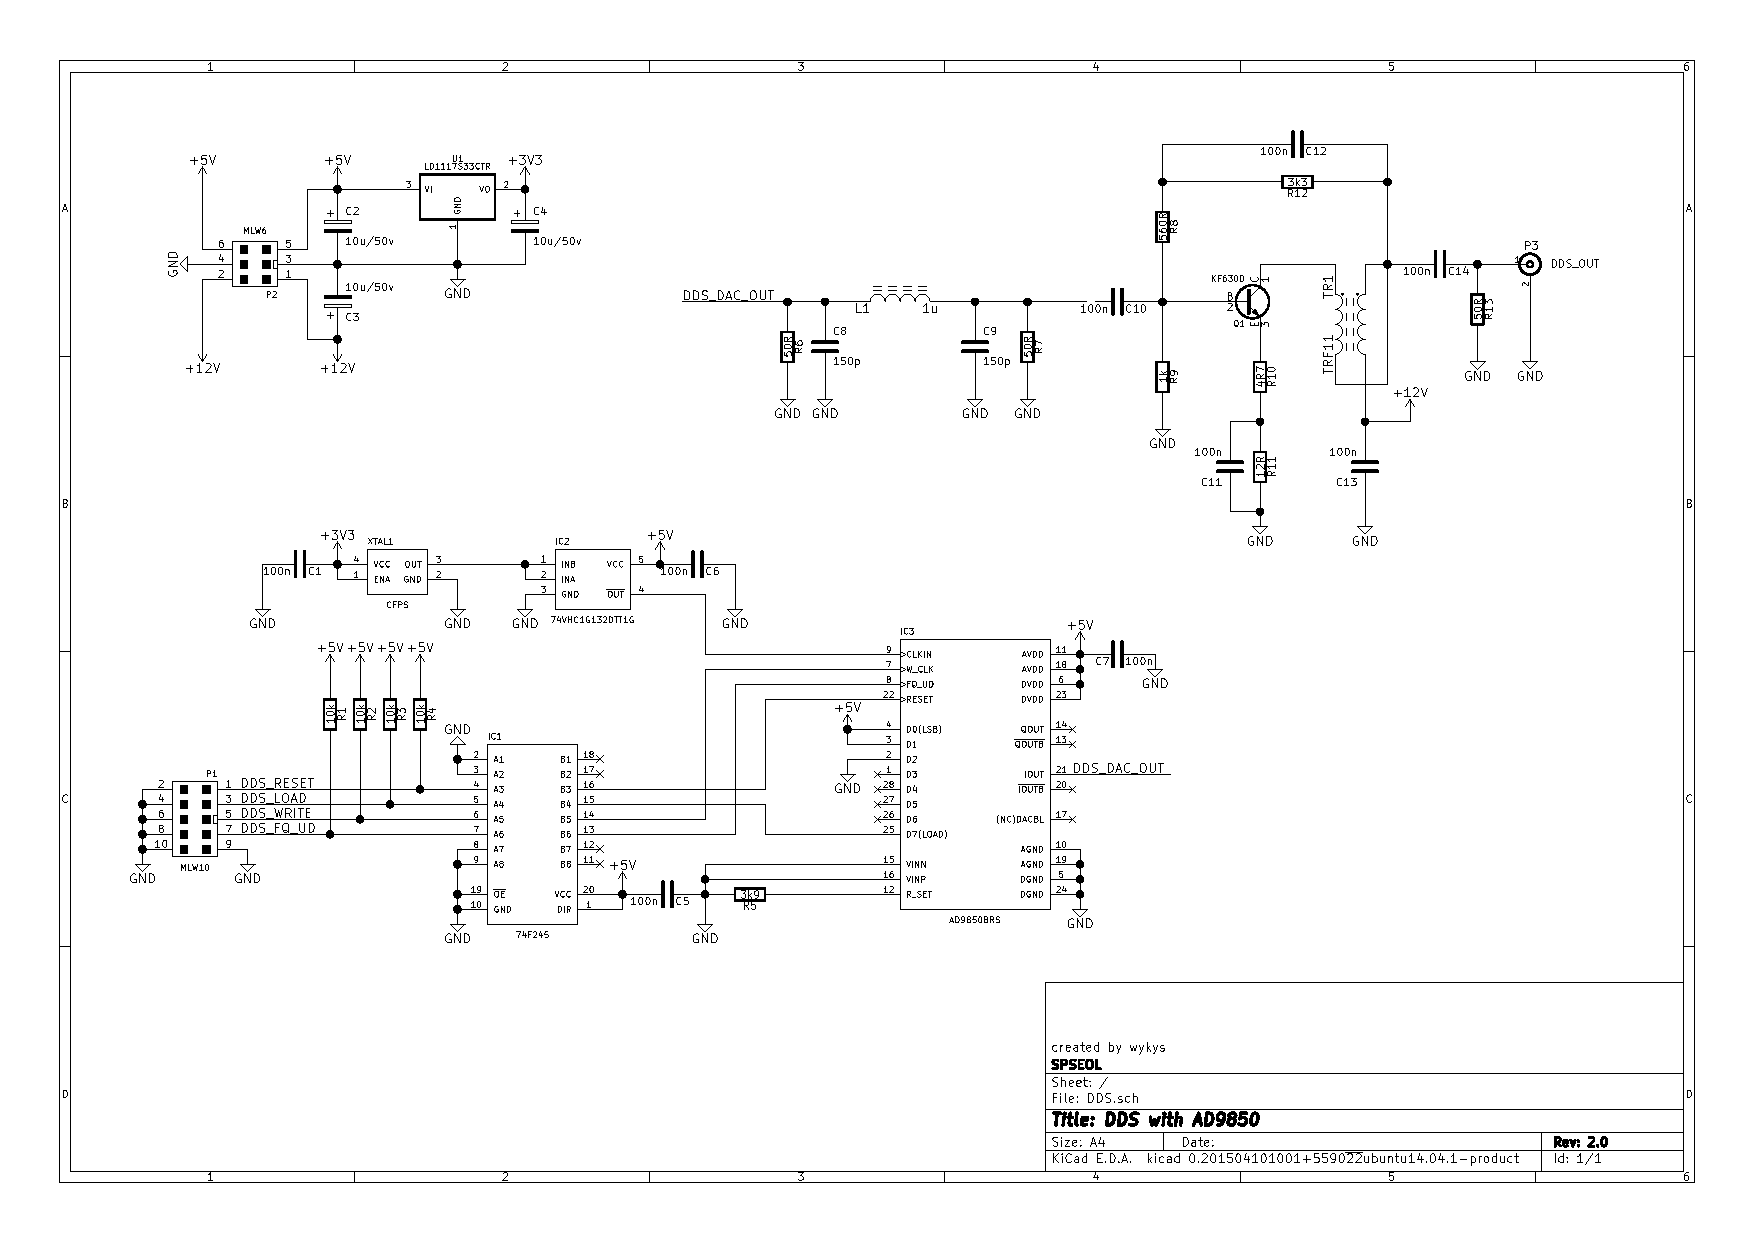
\includegraphics[height=\textwidth]{img/lo/sch.pdf}
		\caption{Schéma zapojení řídící jednotky}	
	\end{figure}
\end{landscape}
%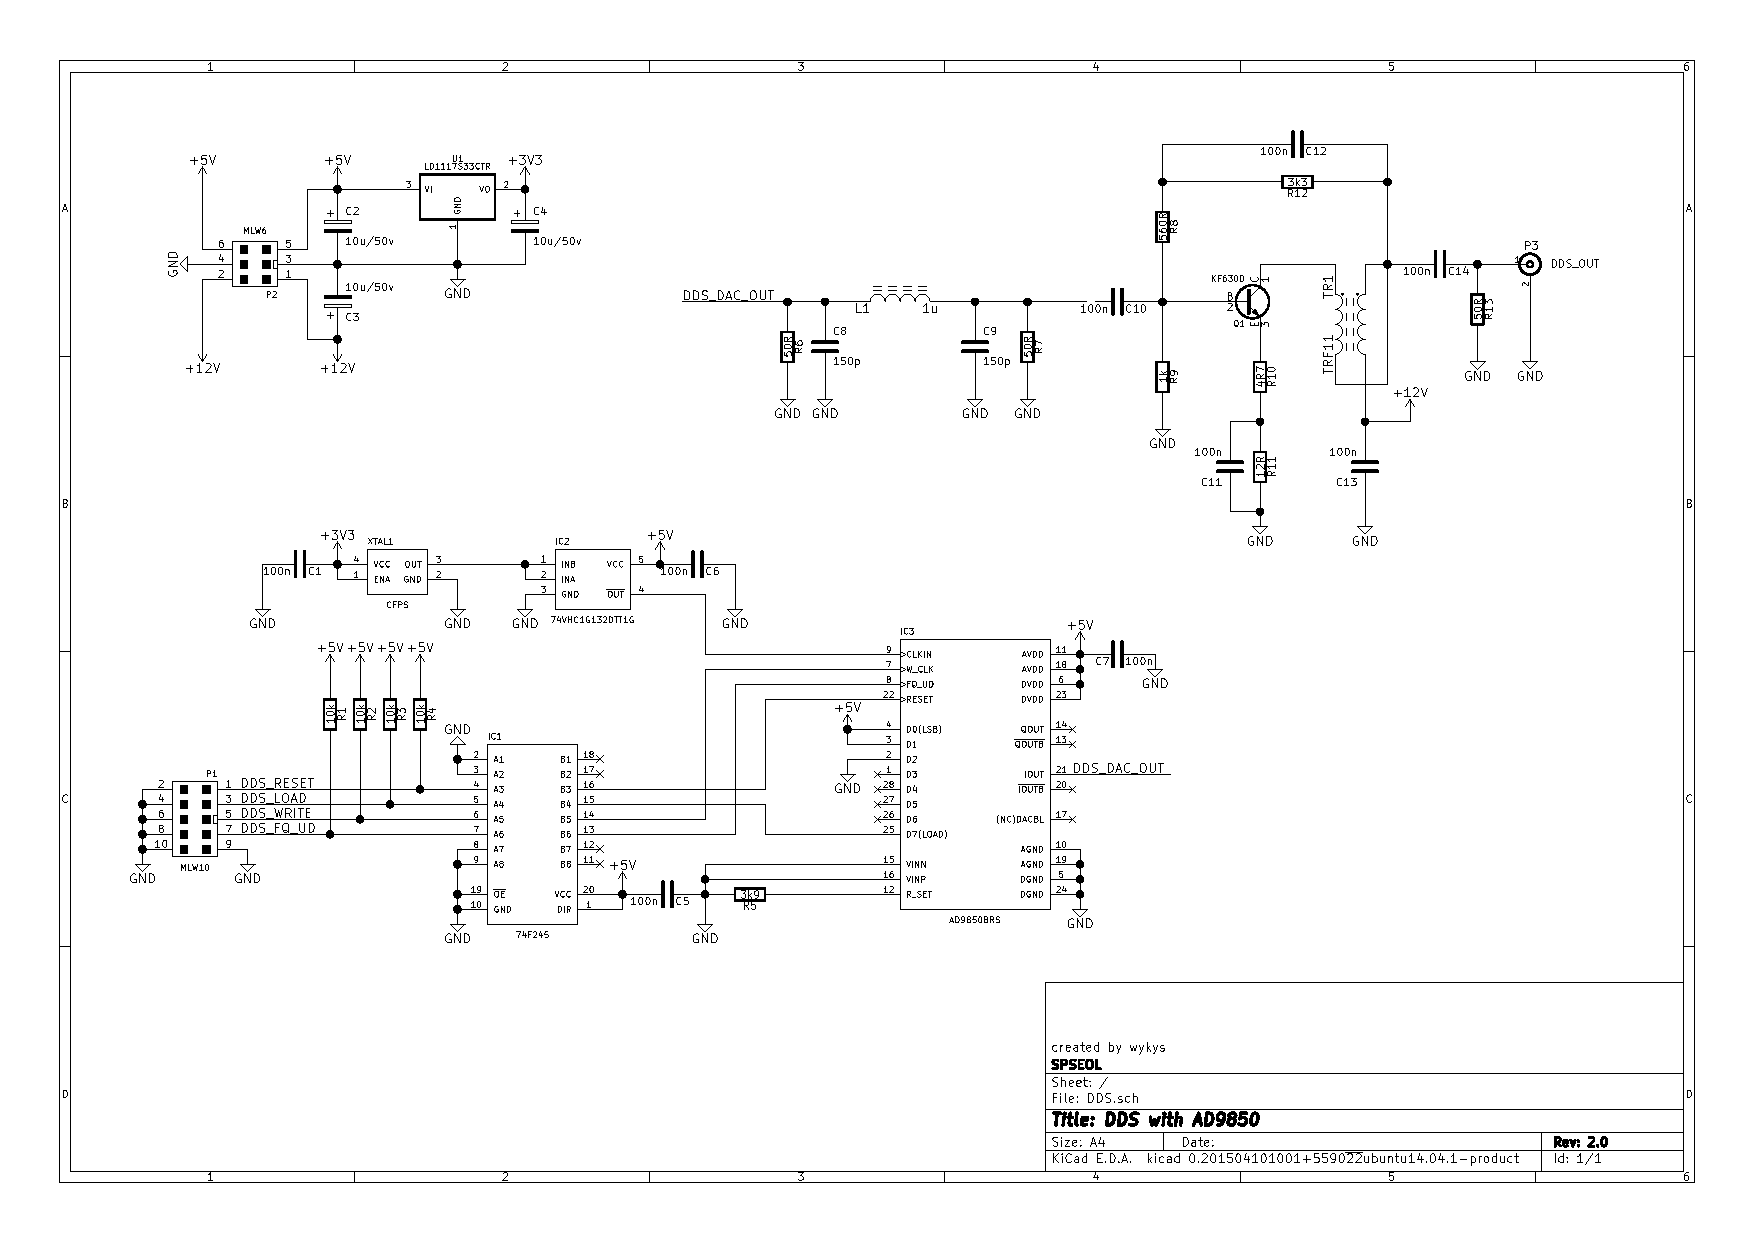
\includepdf[landscape=true]{img/lo/sch.pdf}

% DPS
\begin{figure}[H]
	\centering
	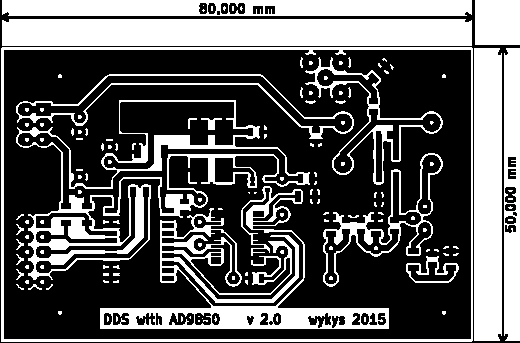
\includegraphics[width=160mm]{img/lo/cu_b.pdf}
	\caption{Deska plošného spoje lokálního oscilátoru, strana spojů}    		
\end{figure}

% os f
\begin{figure}[H]
	\centering
	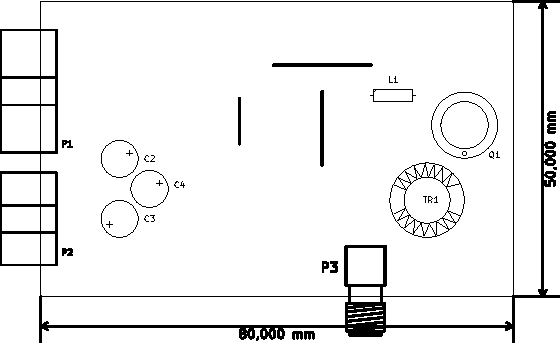
\includegraphics[width=160mm]{img/lo/os_f.pdf}
	\caption{Osazovací plán lokálního oscilátoru, strana součástek}    		
\end{figure}

% os b
\begin{figure}[H]
	\centering
	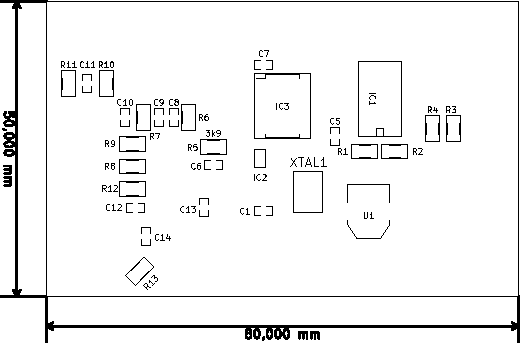
\includegraphics[width=120mm]{img/lo/os_b.pdf}
	\caption{Osazovací plán lokálního oscilátoru, strana spojů}    		
\end{figure}

\begin{table}[H]
	\begin{center}
		\caption{Tabulka použitých součástek pro desku lokálního oscilátoru}
		\label{tab:lo_os}     
		\begin{tabular}[H]{!{\vrule width 1pt}c|c|c|c!{\vrule width 1pt}}
		    \specialrule{1pt}{0pt}{0pt} 
		    \textbf{Určovatel}	&	\textbf{Pouzdro}	&	\textbf{Množství}	&	\textbf{Určení}	\\\specialrule{1pt}{0pt}{0pt} 			
			C1,C5-C7,C10-C14	&	SMD-0805	&	9	&	100n	\\\hline
			C2,C3,C4	&	Elko\_vert\_11.2x6.3mm\_RM2.5	&	3	&	10u/50v	\\\hline
			C8,C9	&	SMD-0805	&	2	&	150p	\\\hline
			IC1	&	SO-20-L	&	1	&	74F245	\\\hline
			IC2	&	SOT-23-5	&	1	&	74VHC1G132DTT1G	\\\hline
			L1	&	R3-LARGE\_PADS	&	1	&	1u	\\\hline
			Q1	&	TO5	&	1	&	KF630D	\\\hline
			R1,R2,R3,R4	&	R\_1206	&	4	&	10k	\\\hline
			R5	&	R\_1206	&	1	&	3k9	\\\hline
			R6,R7,R13	&	R\_1206	&	3	&	50R	\\\hline
			R8	&	R\_1206	&	1	&	560R	\\\hline
			R9	&	R\_1206	&	1	&	1k	\\\hline
			R10	&	R\_1206	&	1	&	4R7	\\\hline
			R11	&	R\_1206	&	1	&	12R	\\\hline
			R12	&	R\_1206	&	1	&	3k3	\\\hline
			TR1	&	Amidon-T44-2	&	1	&	TRF11	\\\hline
			U1	&	SOT-223	&	1	&	LD1117S33CTR	\\\hline
			P3	&	MCX	&	1	&	DDS\_OUT	\\\hline
			P1	&	vasch\_strip\_5x2\_90	&	1	&	MLW10	\\\hline
			P2	&	vasch\_strip\_3x2\_90	&	1	&	MLW6	\\\hline
			M1,M2,M3,M4	&	M3	&	4	&	M3	\\\hline
			IC3	&	SSOP-28	&	1	&	AD9850BRS	\\\hline
			XTAL1	&	SMD7x5	&	1	&	CFPS	\\\specialrule{1pt}{0pt}{0pt} 
		\end{tabular}	 
	\end{center}
\end{table}

